% !TEX program = xelatex
\documentclass[11pt, aspectratio=169]{beamer}
\usetheme{metropolis}
\useoutertheme{metropolis}
\useinnertheme{metropolis}
\usecolortheme{metropolis}
\usefonttheme{professionalfonts} 

\usepackage{kotex}
\usepackage{tikz}
% [!중요!] TikZ 라이브러리 추가 (cloud 모양 등 사용을 위해 필수)
\usetikzlibrary{shapes, arrows, positioning, shadows}
\usepackage{graphicx, caption, hyperref, fontawesome5}
\usepackage{subcaption}

% [수식 및 폰트 설정 - 기존 파일 그대로 유지]
\usepackage{amsmath}
\usepackage[math-style=ISO, bold-style=ISO]{unicode-math}
\usefonttheme{professionalfonts}

% [캡션 스타일 설정]
% 1. 캡션 폰트: 굵게(bold) 제거(\mdseries), 크기는 약간 작게(\small)
\setbeamerfont{caption}{series=\mdseries, size=\small}
\setbeamerfont{caption name}{series=\mdseries}
% 2. 캡션 번호 붙이기 (Figure 1: ...)
\setbeamertemplate{caption}[numbered]
% 3. 캡션 레이블 구분자 (Figure 1. Caption)
\setbeamertemplate{caption label separator}[period]

% [중요] 그림 경로 수정 (슬라이드 폴더 기준 2단계 위로)
\graphicspath{ {./} {../../assets/} {../assets/} }

%%%%%%%%%%%%%%%%%%%%%%%%%%%%%%%%%%%%%%%%%%%%%
%%%%%%%%%%%%%%%%%%%%%%%%%%%%%%%%%%%%%%%%%%%%%%
\title{Communication Theory - 2026}
\subtitle{Chapter 2. Signals and Signal Space}
\date{\today}
\author{
    이 경 근 \\
    {\tiny
        % \texorpdfstring{문서에 보일 내용}{PDF 속성에 들어갈 텍스트(특수문자 제외)}
        \texorpdfstring{\raisebox{-0.1ex}{\scalebox{0.85}{\faEnvelope}}}{} \href{mailto:infosec@knu.ac.kr}{infosec@knu.ac.kr} \quad 
        \texorpdfstring{\scalebox{0.95}{\faLinkedin}}{} \scalebox{0.9}{\href{https://www.linkedin.com/in/Kenny-0633-Lee}{Kenny-0633-Lee}}
    }
}
\institute{EE / KNU}
%%%%%%%%%%%%%%%%%%%%%%%%%%%%%%%%%%%%%%%%%%%%%
%%%%%%%%%%%%%%%%%%%%%%%%%%%%%%%%%%%%%%%%%%%%%
% [Font Settings] Project-Local Fonts (Perfect Stability)
\usepackage{fontspec}

% 시스템 폰트가 아니라, ./fonts 폴더의 파일을 직접 사용합니다.
\setmainfont{NotoSansKR-Regular.ttf}[
    Path = ../../fonts/,             % 폰트 파일 위치
    BoldFont = NotoSansKR-Bold.ttf,
    AutoFakeSlant = 0.2          % 이탤릭 강제 구현
]
\setsansfont{NotoSansKR-Regular.ttf}[
    Path = ../../fonts/,
    BoldFont = NotoSansKR-Bold.ttf,
    AutoFakeSlant = 0.2
]
\setmainhangulfont{NotoSansKR-Regular.ttf}[
    Path = ../../fonts/,
    BoldFont = NotoSansKR-Bold.ttf,
    AutoFakeSlant = 0.2
]
\setsanshangulfont{NotoSansKR-Regular.ttf}[
    Path = ../../fonts/,
    BoldFont = NotoSansKR-Bold.ttf,
    AutoFakeSlant = 0.2
]

% 수식 폰트 설정
\setmathfont{Fira Math}
\setmathfont[range={up, bfup}, Scale=MatchLowercase, Path = ../../fonts/]{NotoSansKR-Regular.ttf}
\setmathfont[range={it, bfit}, Scale=MatchLowercase, FakeSlant=0.2, Path = ../../fonts/]{NotoSansKR-Regular.ttf}
%%%%%%%%%%%%%%%%%%%%%%%%%%%%%%%%%%%%%%%%%%%%%
%%%%%%%%%%%%%%%%%%%%%%%%%%%%%%%%%%%%%%%%%%%%%
%%%%%%%%%%%%%%%%%%%%%%%%%%%%%%%%%%%%%%%%%%%%%

\begin{document}

% #1. Title Page
\begin{frame}[plain]
    \titlepage
\end{frame}

% #2. Intro: The Black Box
\begin{frame}{Introduction: The Black Box}
    \begin{columns}
        \begin{column}{0.4\textwidth}
            \LARGE
            \centering
            \textbf{Smartphone}
            
            \vspace{1cm}
            \normalsize
            \textit{"We use it every day,\\but how does it work?"}
        \end{column}
        \begin{column}{0.6\textwidth}
            \begin{block}{The Physical Question}
                여러분이 카카오톡 \textbf{[전송]} 버튼을 누를 때, \\
                0과 1의 데이터는 어떻게 \textbf{물리적인 파동(Wave)}이 되어 \\
                공기 중으로 날아가는가?
            \end{block}
            \vspace{0.3cm}
            \small \faArrowRight \ 본 강의는 그 \textbf{"물리적 변환(Transformation)"}의 과정을 배웁니다.
        \end{column}
    \end{columns}
\end{frame}

% #3. The Roadmap (Block Diagram)
\begin{frame}{Course Roadmap: The Communication System}
    % Lathi 교재의 블록 다이어그램을 개념적으로 설명
    \centering
    \begin{tikzpicture}[node distance=2cm, auto, thick]
        % TikZ로 간단한 블록 다이어그램 그리기 (이미지 대체 가능)
        \node (tx) [draw, rectangle, fill=orange!10, minimum height=1cm] {Transmitter};
        \node (ch) [draw, cloud, fill=blue!10, right of=tx, node distance=4cm, minimum height=1cm] {Channel};
        \node (rx) [draw, rectangle, fill=green!10, right of=ch, node distance=4cm, minimum height=1cm] {Receiver};
        
        \draw[->] (tx) -- node[above] {\small Signal} (ch);
        \draw[->] (ch) -- node[above] {\small + Noise} (rx);
    \end{tikzpicture}
    
    \vspace{1cm}
    \begin{itemize}
        \item \textbf{Ch 1-3:} 신호와 시스템 (Signals) \hfill \textit{"Language"}
        \item \textbf{Ch 4-5:} 아날로그 통신 (Modulation) \hfill \textit{"Transmission"}
        \item \textbf{Ch 6-7:} 디지털 통신 (Digital/Noise) \hfill \textit{"Robustness"}
    \end{itemize}
\end{frame}

% #4. Ch 1-3 Preview
\begin{frame}{Part 1. Signals (Ch 1-3)}
    \framesubtitle{The Language of Communication: Frequency}
    
    \begin{figure}
        \centering
        \begin{subfigure}{0.32\textwidth}
            \includegraphics[width=\linewidth]{fourier_step_1}
            \caption{N=1}
        \end{subfigure}
        \hfill
        \begin{subfigure}{0.32\textwidth}
            \includegraphics[width=\linewidth]{fourier_step_5}
            \caption{N=5}
        \end{subfigure}
        \hfill
        \begin{subfigure}{0.32\textwidth}
            \includegraphics[width=\linewidth]{fourier_step_29}
            \caption{Square Wave}
        \end{subfigure}
        \caption{Fourier Series: 모든 신호는 사인파의 합이다.}
    \end{figure}
    
    \begin{itemize}
        \item 복잡한 정보를 주파수(Frequency) 성분으로 분해하는 법을 배웁니다.
    \end{itemize}
\end{frame}

% #5. Ch 4-5 Preview
\begin{frame}{Part 2. Analog Modulation (Ch 4-5)}
    \framesubtitle{Moving the Spectrum}
    
    \begin{columns}
        \begin{column}{0.5\textwidth}
            \centering
            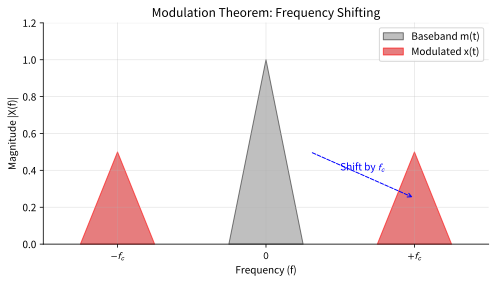
\includegraphics[width=0.95\textwidth]{fig_03_am_shift}
            \vspace{0.2cm}
            \small \textbf{AM (Amplitude Modulation)} \\
            주파수 이사(Frequency Shifting)
        \end{column}
        \begin{column}{0.5\textwidth}
            \centering
            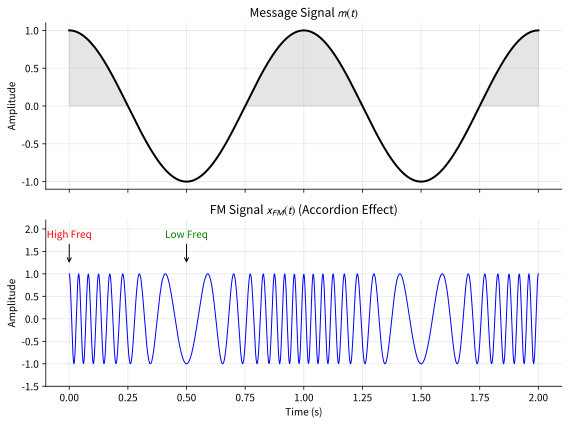
\includegraphics[width=0.95\textwidth]{fig_04_fm_accordion}
            \vspace{0.2cm}
            \small \textbf{FM (Frequency Modulation)} \\
            아코디언 효과 (Noise Immunity)
        \end{column}
    \end{columns}
\end{frame}

% #6. Ch 6-7 Preview
\begin{frame}{Part 3. Digital Communication (Ch 6-7)}
    \framesubtitle{Surviving the Noise}
    
    \begin{columns}
        \begin{column}{0.6\textwidth}
            \centering
            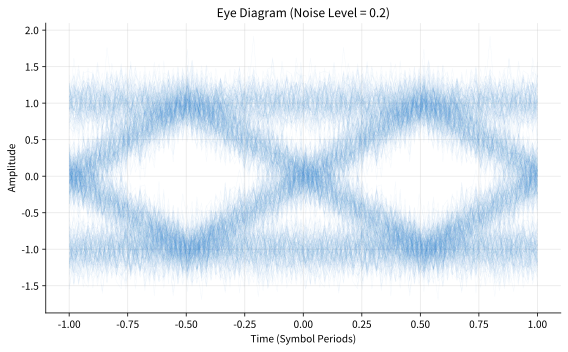
\includegraphics[width=0.9\textwidth]{fig_05_eye_diagram}
        \end{column}
        \begin{column}{0.4\textwidth}
            \textbf{The Eye Diagram}
            \vspace{0.5cm}
            \begin{itemize}
                \item 0과 1을 아날로그 파형에 싣는 법
                \item 잡음(Noise) 속에서 에러 없이 복구하는 법
                \item \textit{"통신 엔지니어는 신호의 눈(Eye)을 뜨게 만드는 사람이다."}
            \end{itemize}
        \end{column}
    \end{columns}
\end{frame}

% #7. Methodology
\begin{frame}{Methodology: Theory meets Code}
    \begin{columns}
        \begin{column}{0.5\textwidth}
            \begin{block}{Textbook (Theory)}
                \[ C = B \log_2 \left( 1 + \frac{S}{N} \right) \]
                수학적 엄밀함을 배웁니다.
            \end{block}
        \end{column}
        \begin{column}{0.5\textwidth}
            \begin{block}{Python (Engineering)}
                \texttt{>>> import numpy as np} \\
                \texttt{>>> plt.plot(t, signal)} \\
                이론을 코드로 검증합니다.
            \end{block}
        \end{column}
    \end{columns}
    
    \vspace{0.5cm}
    \centering
    \faPython \ \textbf{모든 주요 이론은 Python 시뮬레이션 과제가 제공됩니다.}
\end{frame}

% #8. Outro: Starlink
\begin{frame}{Vision: From Textbook to Universe}
    \framesubtitle{Why we learn this?}
    
    \begin{columns}
        \begin{column}{0.6\textwidth}
            % 스타링크 이미지가 있다면 넣고, 없으면 텍스트로 대체
            \centering
            \LARGE \faSatellite \ \faGlobe
            \vspace{0.5cm}
            \normalsize
            \textbf{SpaceX Starlink}
        \end{column}
        \begin{column}{0.4\textwidth}
            \textbf{Advanced Application}
            \begin{itemize}
                \item \textbf{Doppler Effect:} \\
                위성의 빠른 이동 속도 보정 \\
                (Related to Ch 4. FM)
                \item \textbf{Link Budget:} \\
                우주 잡음 극복 설계 \\
                (Related to Ch 5. Noise)
            \end{itemize}
        \end{column}
    \end{columns}
    
    \vspace{0.5cm}
    \centering
    \textit{"기본 이론(Fundamentals)이 미래 기술의 기반입니다."}
\end{frame}

% #9. Closing
\begin{frame}[plain]
    \centering
    \LARGE
    \textbf{Questions?}
    
    \vspace{1cm}
    \normalsize
    See you in the next class.
    
    \vspace{0.5cm}
    \small
    \faEnvelope \ infosec@knu.ac.kr
\end{frame}

\end{document}